Dans cet exercice l'unité est le centimètre.

On considère une pyramide à base carrée SABCD comme dans la figure ci-dessous.

\begin{center}
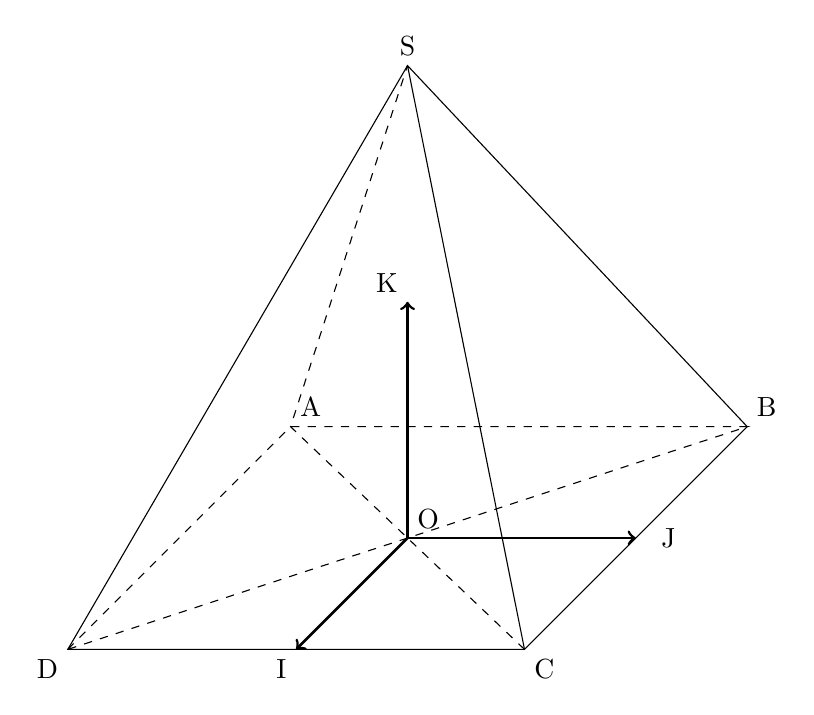
\begin{tikzpicture}[x=(225:20mm),y=(0:29mm),z=(90:30mm)]
	\coordinate (A) at (-1,-1,0);\node[above right] at (A) {A};
	\coordinate (B) at (-1,1,0); \node[above right] at (B) {B};
	\coordinate (C) at (1,1,0); \node[below right] at (C) {C};
	\coordinate (D) at (1,-1,0); \node[below left] at(D) {D};
	\coordinate (S) at (0,0,2); \node[above] at(S) {S};
	\coordinate (O) at (0,0,0); \node[above right] at(O) {O};
	\coordinate (I) at (1,0,0); \node[below left] at(I) {I};
	\coordinate (J) at (0,1,0); \node[right=2mm] at(J) {J};
	\coordinate (K) at (0,0,1); \node[above left] at(K) {K};
	\draw[dashed] (D)--(A)--(B)--cycle
	(C)--(A)--(S);
	\draw (D)--(C)--(B)--(S)--cycle
	(S)--(C);
	\draw[->,line width=1pt] (O)--(I);
	\draw[->,line width=1pt] (O)--(J);
	\draw[->,line width=1pt] (O)--(K);
	\end{tikzpicture}
\end{center}
















Dans cette figure :

\begin{itemize}
\item AB = BC = CD = DA = OS = 2~cm ;
\item I est le milieu de [CD], J le milieu de [BC] et K le milieu de [OS].
\end{itemize}

L'espace est muni du repère orthonormé $\left(\mathrm{O}; \vectt{OI}, \vectt{OJ}, \vectt{OK}\right)$.

On admet que B$(-1~;~1~;~0)$, C$(1~;~1~;~0)$, et S$(0~;~0~;~2)$.

\medskip

Les \textbf{parties A} et \textbf{B} sont indépendantes.

\textbf{Partie A}

\begin{enumerate}
\item Donner les coordonnées des points A et D.
\item Calculer le produit scalaire $\vectt{SC}\cdot\vectt{SB}$.
\item En déduire la mesure de l'angle $\widehat{\mathrm{BSC}}$ arrondie au dixième de degré près.
\end{enumerate}

\textbf{Partie B}

On se propose dans cette partie de déterminer la distance du point O au plan (SBC).

\begin{enumerate}
\item Soit $\vect{n}$ le vecteur de coordonnées $\begin{pmatrix} 0\\ 2\\ 1\\ \end{pmatrix}$.
	\begin{enumerate}
		\item Justifier que le vecteur $\vect{n}$ est normal au plan (SBC).
		\item En déduire qu'une équation cartésienne du plan (SBC) est \quad $2 y+z-2=0$.
	\end{enumerate}
	\item On note H le projeté orthogonal du point O sur le plan (SBC).
		\begin{enumerate}
			\item a. Justifier qu'une représentation paramétrique de la droite (OH) est :
			\[\begin{cases}
			x =0\\
			y =2t\\
			z =t\\
			\end{cases}\text{ avec } t \in \R.\]
			\item Calculer les coordonnées du point H.
			\item En déduire que la distance du point O au plan (SBC) est égale à $\dfrac{2 \sqrt{5}}{5}$~cm.
		\end{enumerate}
	\end{enumerate}

\textbf{Partie C}

On se propose ici de retrouver le résultat de la \textbf{partie B} par une autre méthode.

\begin{enumerate}
\item On rappelle que le volume d'une pyramide est donné par :

\[V =\dfrac{1}{3} \times \text{ aire de la base} \times \text{hauteur}\]

	\begin{enumerate}
		\item Calculer le volume de la pyramide SABCD.
		\item En déduire que le volume de la pyramide OCBS est égal à $\dfrac{2}{3}$~cm\up{3}.
	\end{enumerate}
\item Déterminer l'aire du triangle SBC.
\item Déduire des questions précédentes que la distance du point O au plan (SBC) est égale à $\dfrac{2 \sqrt{5}}{5}$~cm.
\end{enumerate}
